
% This LaTeX was auto-generated from MATLAB code.
% To make changes, update the MATLAB code and republish this document.

\documentclass{article}
\usepackage{graphicx}
\usepackage{color}

\sloppy
\definecolor{lightgray}{gray}{0.5}
\setlength{\parindent}{0pt}

\begin{document}

    
    \begin{verbatim}
close all, clear all, clc;
tx = 0:1:10;
%Generating p(t)
for t = 0:1:10
    t_ = t*(1/10);
    if t <= 5
        pt(t+1) = 1*t_;
    else
        pt(t+1) = 1*(1-t_);
    end
end

figure(1);
plot(pt);
title(' Figure1 : p(t)');
xlabel('x[n]');
ylabel('amplitude');

DFT_11 = abs(fftshift(fft(pt,11)));

figure(2);
stem(DFT_11);
title(' Figure2 : DFT for L = 11');
xlabel('X(k)');
ylabel('amplitude');

figure(3);
IDFT_11 = ifft((fft(pt,11)),11);
stem(IDFT_11);
title('  Figure3 : IDFT for L = 11');
xlabel('x[n]');
ylabel('amplitude');

%L = 22
DFT_22 = abs(fftshift(fft(pt,22)));

figure(4);
stem(DFT_22);
title(' Figure4 : DFT for L = 22');
xlabel('X(k)');
ylabel('amplitude');

figure(5);
IDFT_22 = ifft((fft(pt,22)),22);
stem(IDFT_22);
title(' Figure5 : IDFT for L = 22');
xlabel('x[n]');
ylabel('amplitude');


%L = 33
DFT_33 = abs(fftshift(fft(pt,33)));

figure(6);
stem(DFT_33);
title(' Figure6 : DFT for L = 33');
xlabel('X(k)');
ylabel('amplitude');

figure(7);
IDFT_33 = ifft((fft(pt,33)),33);
stem(IDFT_33);
title(' Figure7 : IDFT for L = 33');
xlabel('x[n]');
ylabel('amplitude');
\end{verbatim}

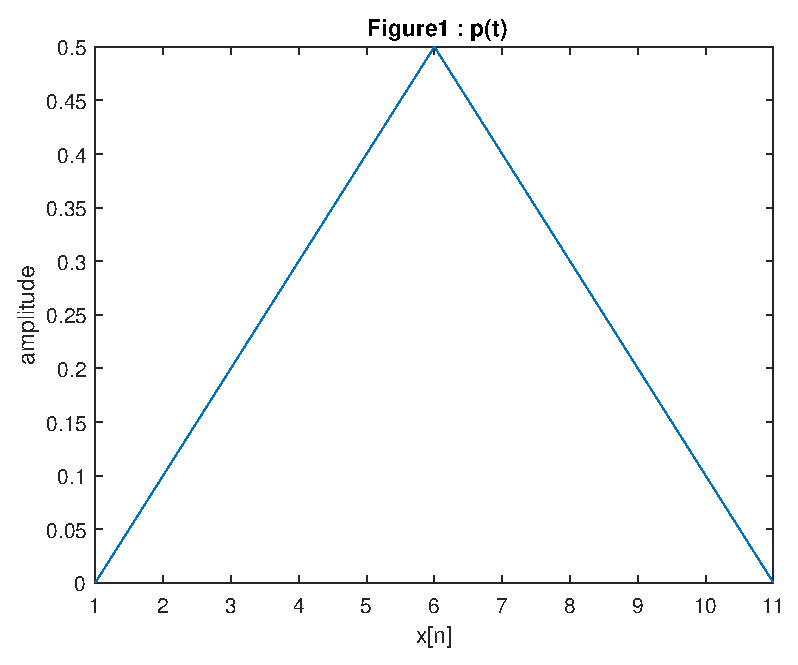
\includegraphics [width=4in]{HW4_01.eps}

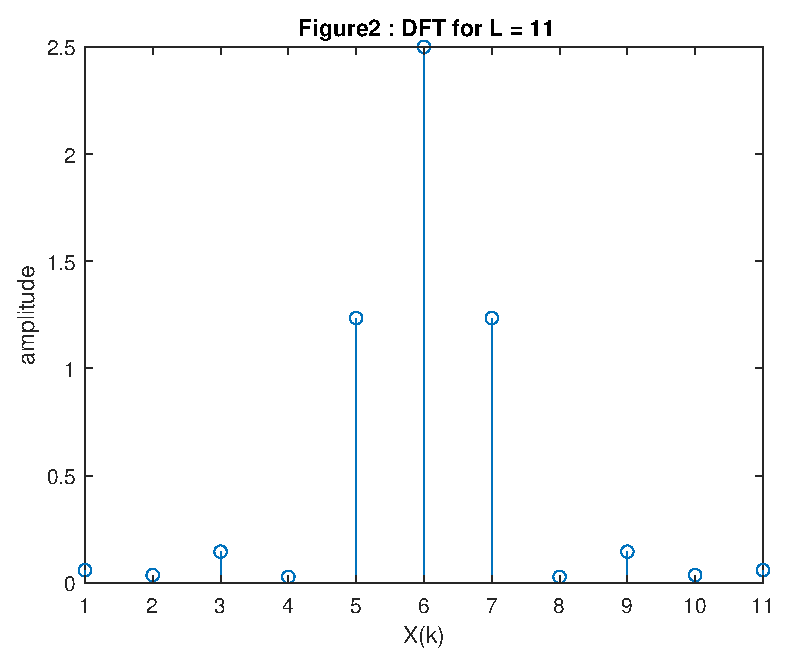
\includegraphics [width=4in]{HW4_02.eps}

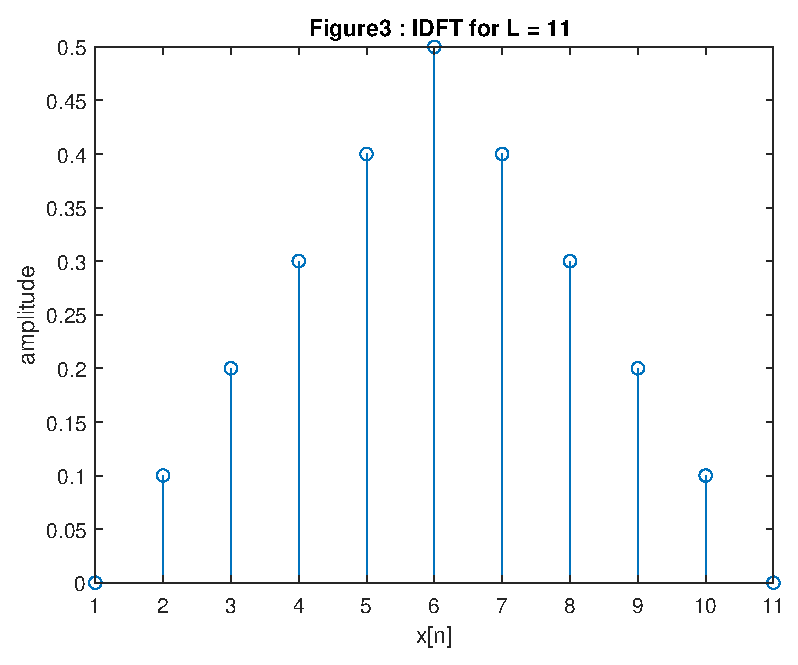
\includegraphics [width=4in]{HW4_03.eps}

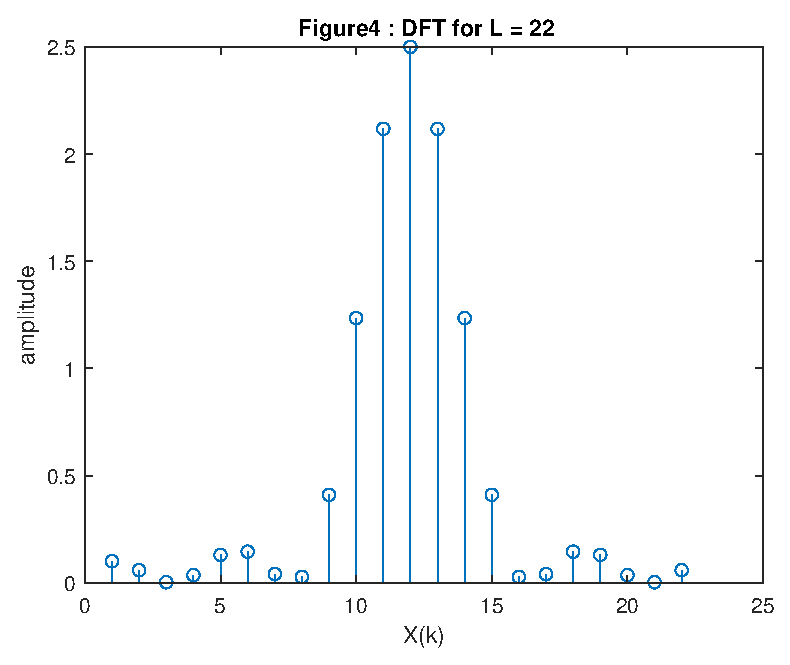
\includegraphics [width=4in]{HW4_04.eps}

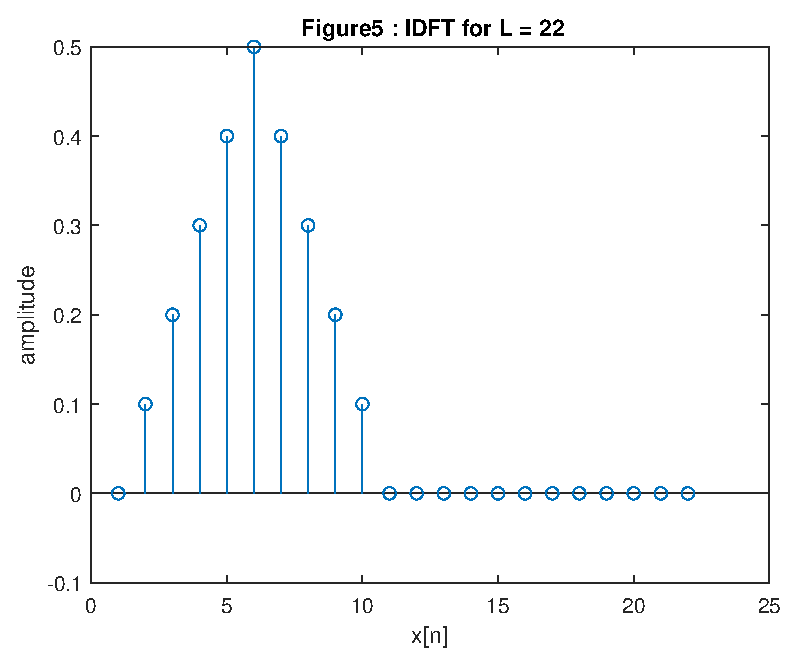
\includegraphics [width=4in]{HW4_05.eps}

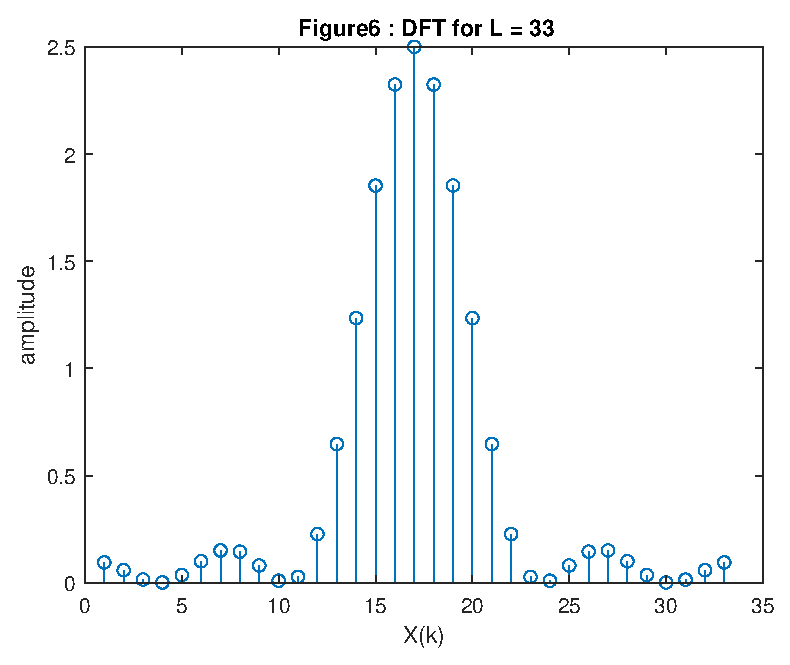
\includegraphics [width=4in]{HW4_06.eps}

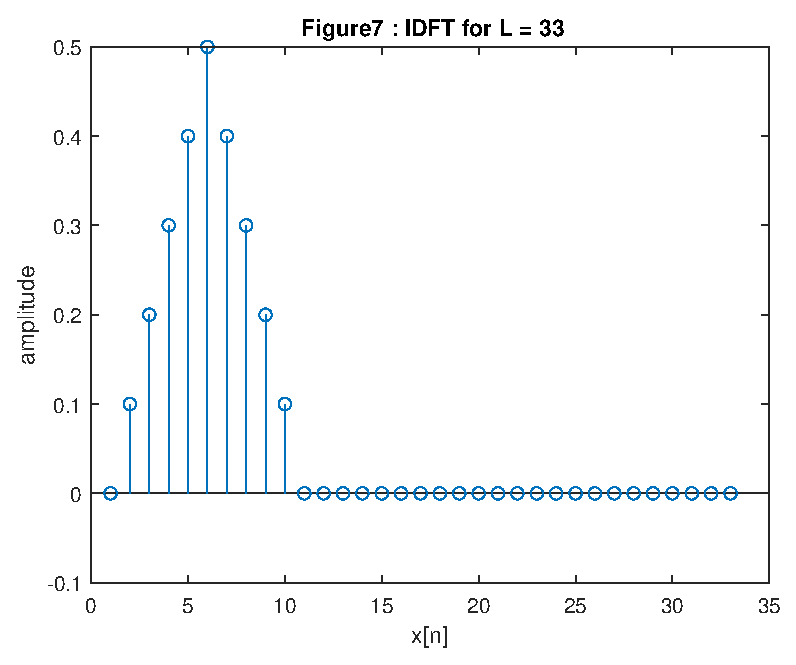
\includegraphics [width=4in]{HW4_07.eps}



\end{document}

